\renewcommand{\thechapter}{\arabic{chapter}}
\setcounter{chapter}{0}

\chapter{La peau et ses lésions}
\label{chap:chapter_1}
\chapterintro
Comme introduction à ces travaux, ce premier chapitre apporte une description de l'organe sujet de cette étude~: la peau. Ainsi, ces quelques pages posent les bases et décrivent pas à pas divers aspects permettant une compréhension sur sa physiologie, son fonctionnement et ses rôles. De plus, cette section est également l'occasion d'aborder les multiples pathologies pouvant altérer cet organe.\par

Dans un premier temps, une explication de ses principales couches et composantes est réalisée par profondeur croissante. Dans un second temps, ce travail consacre une partieà la présentation de quelques unes de ses principales lésions. Par ailleurs, ces pages sont l'occasion d'aborder une première fois le Lentigo, pathologie centrale de cette étude, et tout particulièrement ses formes malignes~: le \acrfull{lm} et le \acrfull{lmm}.\par
\newpage

\section{Présentation, composition et fonctions}
La première section de chapitre dédié à la peau propose d'introduire de manière synthétique la composition et le fonctionnement de cet organe, avant de présenter ses lésions. Ainsi, les différentes couches composant la peau sont abordées par ordre de profondeur croissant lors des prochains paragraphes.\par

\subsection{Présentation}
Le terme "peau" caractérise dans son sens le plus global, l’enveloppe externe propre aux vertébrés. Présente chez l’homme, elle est l’un de ses organes majeurs mais également l’un des plus lourds~: chez un individu adulte d’un poids de \SI{70}{\kilo\gram}, elle représente une surface plane d’environ \SI{2}{\metre\squared}, soit une masse estimée à \SI{5}{\kilo\gram} \cite{McGrath2010}. Son épaisseur diffère selon la zone du corps étudiée~: de \SI{0,5}{\milli\metre} au niveau de zones fines telles que les paupières, à plusieurs centimètres sur les zones adipeuses. La surcharge pondérale influe également de manière importante sur son épaisseur, bien plus élevée chez des personnes souffrant d'obésité.\par

Bien que la peau soit l'un des premiers éléments visible d'un individu, son fonctionnement et ses fonctionnalités sont souvent méconnues par la plupart d’entre nous. Elle assure pourtant des rôles multiples, dont~:
\begin{itemize}
    \item un rôle \textbf{physique}, en apportant une protection contre le monde extérieur,
    \item un rôle \textbf{mécanique}, en limitant la perte d’eau ou en offrant une thermorégulation,
    \item un rôle \textbf{sensoriel}, en permettant l'appréhension de notre monde.
\end{itemize}\par

La dermatologie, branche médicale dédiée à l’étude de la peau, nous permet de mieux comprendre sa composition, son fonctionnement, ses vulnérabilités et permet d’apporter conseils, préventions et traitements dans le cas de certaines pathologies.\par

Cette barrière se décompose en diverses couches fondamentales~: l’épiderme, la membrane basale, le derme et l’hypoderme, dont la représentation est visible sur la \Cref{fig:illustration_skin_kholoski}.\par
\begin{figure}[H]
    \centering
    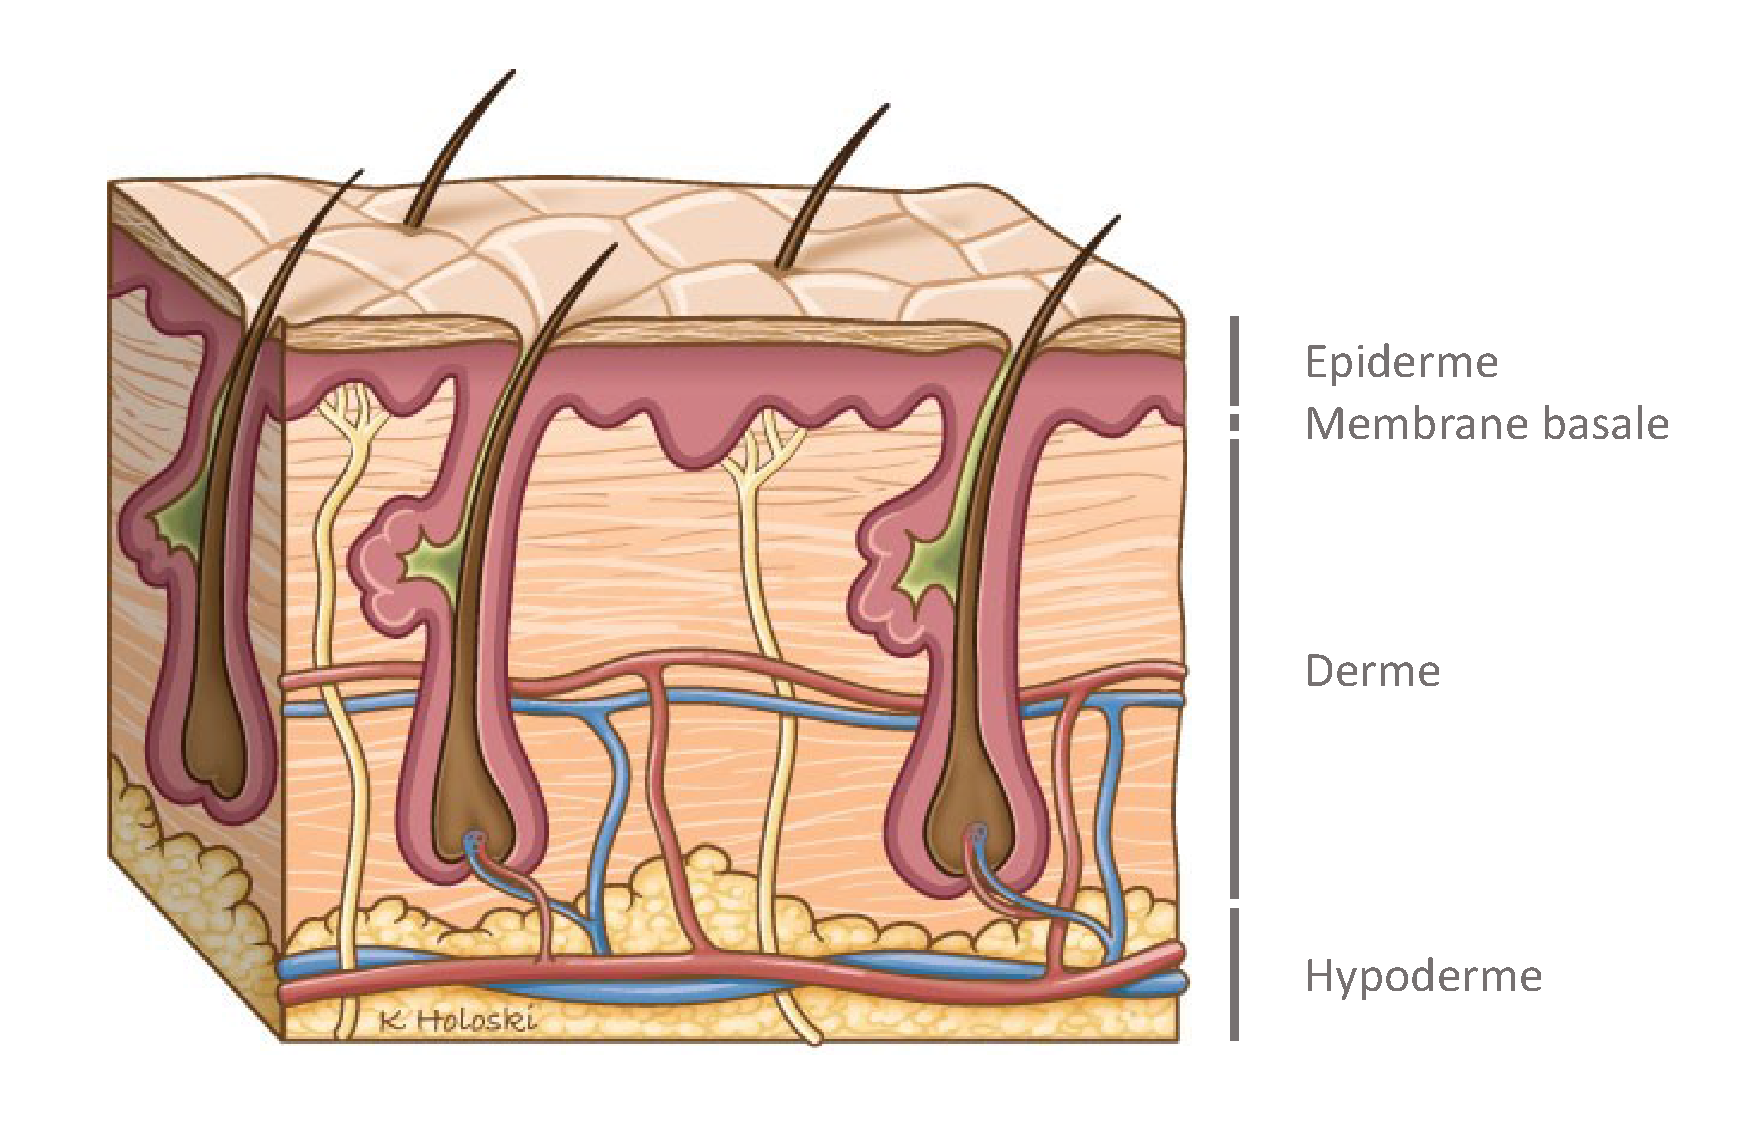
\includegraphics[width=0.6\linewidth]{contents/chapter_1/resources/illustration_skin_kholoski.pdf}
    \caption{Illustration macroscopique de la peau et de ses diverses couches~\textsuperscript{\ref{footnote:illustration_skin_kholoski}}.}
    \label{fig:illustration_skin_kholoski}
\end{figure}\par 

\addtocounter{footnote}{1}
\footnotetext[\thefootnote]{Image source~: Dessin par \href{http://kholoski.com/}{Kellie Holoski} – Illustrateur médical. \label{footnote:illustration_skin_kholoski}}

\subsection{Épiderme}
L’épiderme correspond à la couche superficielle de notre peau et mesure entre \SI{0,01}{\milli\metre} et \SI{0,1}{\milli\metre} d’épaisseur \cite{Sandby-Moller2003}. Un aperçu des différents types de cellules la composant peut être visible sur la \Cref{fig:illustration_epidermis_kholoski}, parmi lesquelles sont recensés~:
\begin{itemize}
    \item les \textbf{kératinocytes}~: des cellules dont le rôle est d'offrir une protection contre l'environnement extérieur et d'apporter une imperméabilité. Elles représentent 90 \% des cellules de l'épiderme.
    \item les \textbf{cellules de Langerhans}~: des cellules dont le rôle est immunitaire.
    \item les \textbf{cellules de Merkel}~: des cellules dont le rôle sensitif.
    \item les \textbf{mélanocytes}~: des cellules dont le rôle est d'assurer la protection contre les rayonnements \gls{uv} par l'apport d'une pigmentation.
\end{itemize}\par

 \begin{figure}[H]
    \centering
    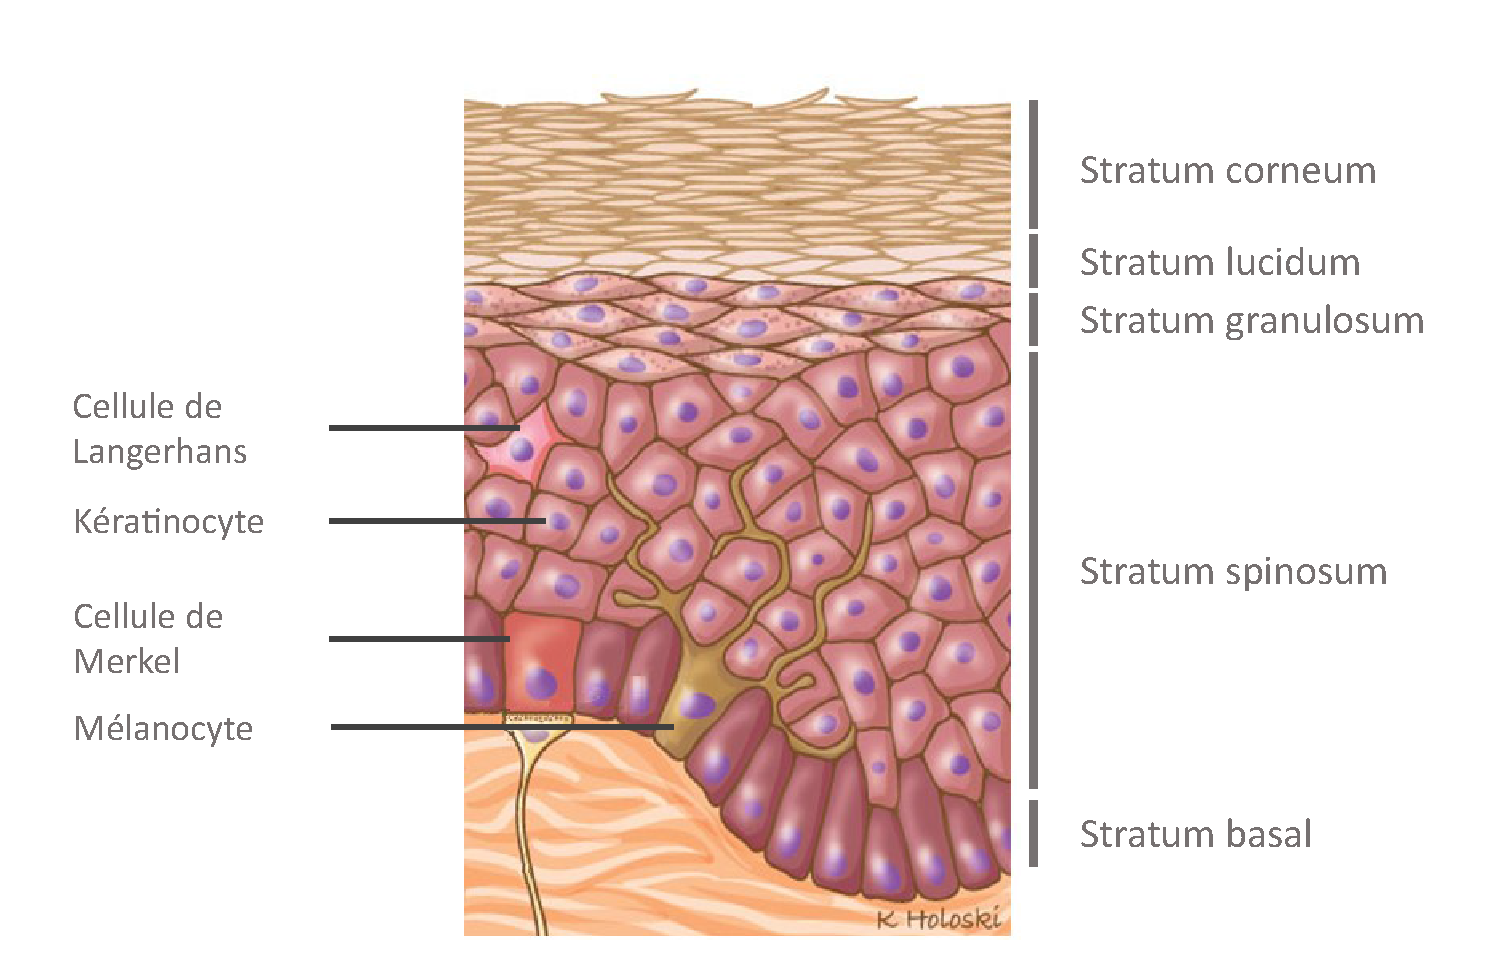
\includegraphics[width=0.9\linewidth]{contents/chapter_1/resources/illustration_epidermis_kholoski.pdf}
    \caption{Illustration des diverses couches de l'épiderme formées par un processus de différenciation ainsi que ses divers composés cellulaires \textsuperscript{\ref{footnote:illustration_epidermis_kholoski}}.}
    \label{fig:illustration_epidermis_kholoski}
\end{figure}\par

\addtocounter{footnote}{1}
\footnotetext[\thefootnote]{Image source~: Dessin par \href{http://kholoski.com/}{Kellie Holoski} – Illustrateur médical. \label{footnote:illustration_epidermis_kholoski}}

Son processus de différenciation des cellules est l’une de ses caractéristiques essentielles. Les kératinocytes, sa principale composante, migrent de la couche inférieure à la couche supérieure en subissant différentes modifications chimiques conduisant à la perte de leur noyau et à la mort de ces cellules. Ce processus porte le nom de kératinisation, et se subdivise en sous couches aux propriétés variées, respectivement par profondeur croissante~: Cornée (Stratum corneum), Transition (Stratum lucidum), Granuleuse (Stratum granulosum), Epineuse (Stratum spinosum), Basale (Stratum basale). Ces différentes couches peuvent être observées sur la \Cref{fig:illustration_epidermis_kholoski}. En fin de parcours, ces cellules perdent leur cohésion dans un processus de desquamation conduisant la peau à se renouveler.\par
\clearpage

\subsection{Jonction dermo-épidermique}
La \gls{dej}, ou encore membrane basale, se situe à la jonction de l’épiderme et du derme, et peut être observée par microscopie optique ou électronique selon l’épaisseur de cette dernière. Son épaisseur, variable selon la zone considérée, est estimée entre \SI{60}{\nano\metre} et \SI{300}{\nano\metre}. 
Cette membrane est scindée en 2 parties~:
\begin{itemize}
\item La lame basale (lamina basalis), divisée en deux couches~: Lamina Lucida et Lamina Densa
\item La lame réticulaire ou zone fibrillaire (lamina reticularis ou fibroreticularis).
\end{itemize}\par
\begin{figure}[H]
    \centering
    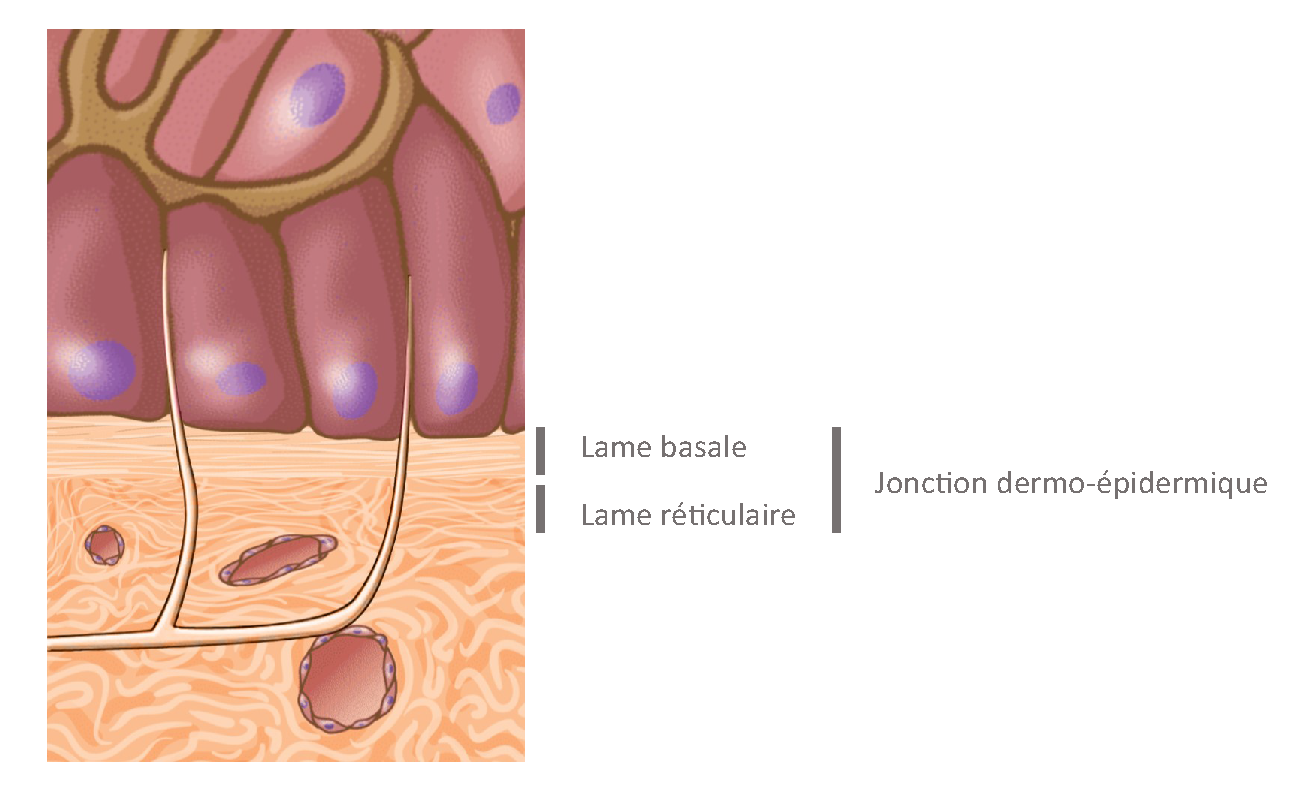
\includegraphics[width=\linewidth]{contents/chapter_1/resources/illustration_basal_basement.pdf}
    \caption{Illustration de la jonction dermo-épidermique \textsuperscript{\ref{footnote:illustration_basal_basement}}. Cette jonction dont le rôle est d'assurer une cohésion entre l'épiderme et le derme peut être subdivisée en deux sous couches~: la lame basale et réticulaire.}
    \label{fig:illustration_basal_basement}
\end{figure}\par

\addtocounter{footnote}{1}
\footnotetext[\thefootnote]{Image source~: Principles of Anatomy and Physiology – John Wiley \& Sons. \label{footnote:illustration_basal_basement}}

Il s’agit d’une zone fibreuse, composée de laminine, de collagène de type III / IV / VI lui conférant entre autres des propriétés de résistance mécanique, voire élastiques. Ces fibres lui permettent d’assurer une cohésion entre épiderme et derme au travers de points d’ancrage. Sa seconde fonction essentielle est au travers d’un mécanisme de régulation des échanges moléculaires, permettant d’assurer la nutrition des cellules de base de l’épiderme. Pour finir, elle possède un rôle de ré-épidermisation fondamentale lors de la cicatrisation.\par
\clearpage

\subsection{Derme}
Le derme est une couche d’une épaisseur estimée comprise entre \SI{0,5}{\milli\metre} et \SI{5}{\milli\metre}, composée majoritairement de collagène à hauteur de 80 \% (sur la matières sèche), et de fibres élastiques \cite{McGrath2010}. Cette couche est traversée par de nombreux éléments dont~: 

\begin{itemize}
    \item des \textbf{vaisseaux sanguins}, qui apportent nutriments
    \item des \textbf{vaisseaux lymphatiques}, qui assurent une fonction immunitaire.
\end{itemize}\par

En outre, cette strate contribue de manière essentielle à des aspects de résistance et de contrainte mécanique de la peau, ainsi qu’aux mécanismes de thermorégulation et de cicatrisation de cette dernière. Enfin, cette couche tient un rôle essentiel dans la perception sensorielle (somesthésie) assurant d’une part des propriétés liées à la pression (mécanorécepteurs) mais également liées à la chaleur (thermorécepteurs). Outre ces fonctions, on lui attribue également un rôle nutritif important de par son irrigation sanguine.\par

La littérature scinde le derme en deux parties majeures, visibles en \Cref{fig:illustration_dermis_kholoski}, dont~:
\begin{itemize}
    \item le \textbf{derme Papillaire} (Papillary dermis), permettant essentiellement la thermorégulation,
    \item le \textbf{derme Réticulaire} (Reticular dermis), assurant la plupart des fonctions mécaniques.
\end{itemize}\par

\begin{figure}[H]
    \centering
    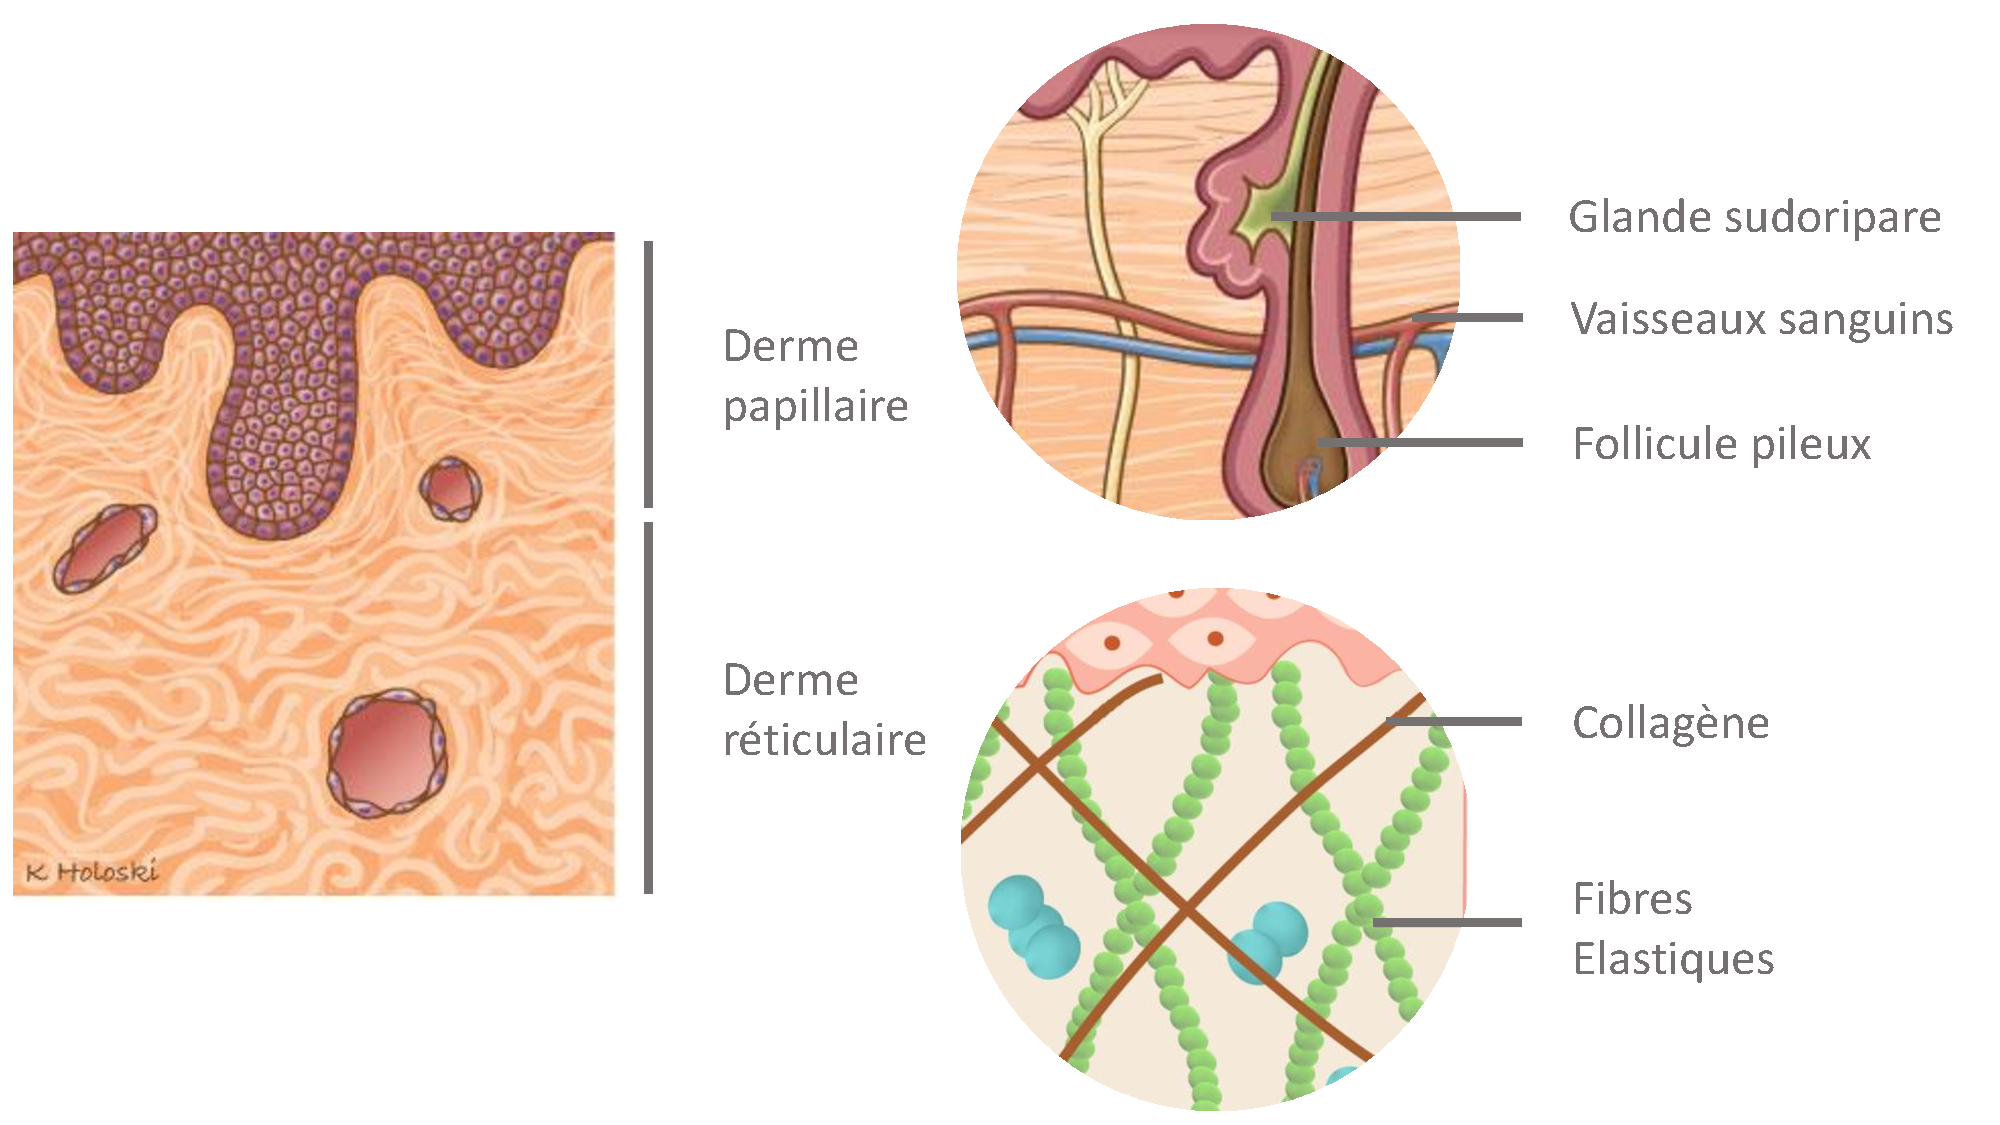
\includegraphics[width=\linewidth]{contents/chapter_1/resources/illustration_dermis_kholoski.pdf}
    \caption{Illustration de représentation du derme \textsuperscript{\ref{footnote:illustration_dermis_kholoski}}. Le derme est subdivisé en deux couches aux propriétés distinctes~: le derme papillaire et réticulaire.}
    \label{fig:illustration_dermis_kholoski}
\end{figure}\par

\addtocounter{footnote}{1}
\footnotetext[\thefootnote]{Image source~: Dessin par \href{http://kholoski.com/}{Kellie Holoski} – Illustrateur médical. \label{footnote:illustration_dermis_kholoski}}
\clearpage

\subsection{Hypoderme}
L’hypoderme, également appelé couche sous-cutanée, est un tissu présent sous le derme composé essentiellement de graisses (adipocytes, cellules spécialisées dans le stockage de graisses). Son épaisseur est extrêmement variable de \SI{0,1}{\centi\metre} à \SI[parse-numbers = false]{plusieurs}{\centi\metre}, selon~:
\begin{itemize}
\item La zone considérée
\item L’âge du patient
\item L’alimentation
\item Les prédispositions génétiques.
\end{itemize}\par

Cette couche de tissu assure diverses fonctions, dont~:
\begin{itemize}
\item Le passage des vaisseaux sanguins et lymphatiques, ainsi que celui des nerfs jusqu’au derme
\item L’interface entre les structures sous cutanées et la peau.
\end{itemize}\par

\subsection{Types de peau}
Il est nécessaire afin de bien aborder ce sujet et ses problématiques, d’être conscient des variations inter individus. Pour répondre partiellement à ces variations, Fitzpatrick a établi une classification des profils type de peau, visant à caractériser leur réaction suite à l’exposition au soleil. Ce travail a également permis de créer une association entre profil type et couleur de peau avant et après exposition au soleil \cite{Fitzpatrick1988}. 
\begin{figure}[H]
    \centering
    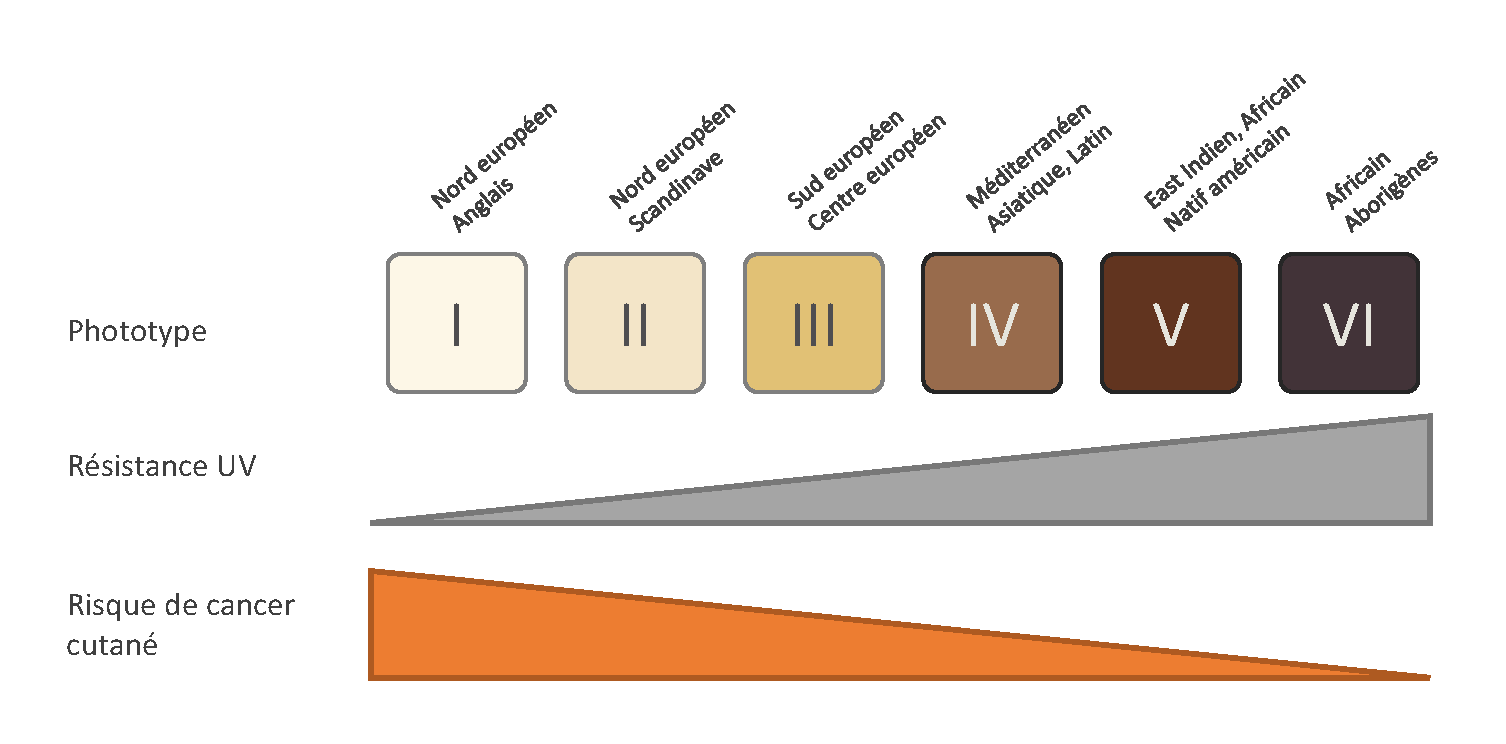
\includegraphics[width=0.8\linewidth]{contents/chapter_1/resources/scheme_fitzpatrick_scale.pdf}
    \caption{Échelle de Fitzpatrick associant type de peau et caractéristiques associées \cite{Fitzpatrick1988}.}
    \label{fig:scheme_fitzpatrick_scale}
\end{figure}
Cet aspect est un élément important à prendre en compte lors de notre appréhension de la problématique. En effet, les travaux d'aide au diagnostic présent dans la littérature ne décrivent pas toujours les types de peau utilisés \cite{Celebi2007,Wiltgen2008,Koller2011}. Néanmoins, les échantillons mis en avant par ces travaux semblent majoritairement axés sur les types I/II de peau. Certaines pathologies sont ainsi plus propices à se développer sur un type de peau en particulier~\cite{Narayanan2010}. De plus, une même pathologie pourra diverger en terme de caractéristiques \cite{Tuma2015}. Nous retrouvons sur la \Cref{fig:scheme_fitzpatrick_scale}, une synthèse visuelle de ces types de peau et de leurs caractéristiques.

\section{Lésions de la peau}
Notre sujet abordant les lésions de la peau, il convient de définir le terme lésion pour bien situer l’objet de notre recherche. Selon PubMed, une lésion « correspond à toute anomalie touchant les tissus d’un organisme, généralement provoquée par une maladie ou par un traumatisme. » \textsuperscript{\ref{footnote:lesion_pubmed}}.\par
\addtocounter{footnote}{1}
\footnotetext[\thefootnote]{Source~: Définition par \href{https://www.ncbi.nlm.nih.gov/pubmedhealth}{PubMed Health}. \label{footnote:lesion_pubmed}}

Les lésions de la peau correspondent à un terme générique caractérisant une partie de la peau ayant, en comparaison de la peau l’entourant, une croissance/apparence ou structure qui diffère. Ces lésions peuvent ainsi être pré-natales ou post-natales, comporter diverses formes et peuvent présenter différents risques.\par

Nous décrivons par le terme « lésion pigmentaire », les lésions affectant la peau présentant des pigmentations liées à la mélanine, au sang, ou de tout autre composant extérieur à la peau. Ces lésions peuvent être d’origine mélanocytaire (Nevus, lentigo, lentigo malin, \ldots) ou non mélanocytaire (nous nous intéresserons aux divers carcinomes lorsque nous aborderons les lésions malignes).\par

Nous traiterons sommairement des lésions de la peau au travers de ces quelques pages. Nous aborderons dans un premier temps les lésions bénignes et nous orienterons dans un second temps ce travail vers les lésions dites malignes. Enfin, nous présenterons le Lentigo, pathologie que nous étudierons dans ce manuscrit.\par

\subsection{Lésions bénignes}
Ces lésions désignent les diverses altérations classées comme sans conséquences graves pour la santé d'un individu, néanmoins ces lésions peuvent présenter un terrain pour des lésions plus dangereuses.\par

L'une des lésions bénignes les plus communes est la tumeur mélanocytaire, à l’apparence de structures souvent circulaires ou ovales présentes en surface de peau chez l’homme. Les naevus sont susceptibles d’évoluer au cours du temps et peuvent rarement aboutir à un mélanome. Ces tumeurs apparaissent pour la plupart d'entre elles durant les trente premières années de vie en moyenne et présentent des couleurs variées, avec des teintes allant d'un rose rougeâtre jusqu'au noir. Voici quelques-unes des catégories et critères associés~:
\begin{itemize}
    \item Nævus commun, ou « grain de beauté » est le plus fréquent et se compose de mélanocytes regroupés en amas.
    \item Nævus atypique, se caractérise la plupart du temps par une pigmentation variable et des bordures irrégulières.
    \item Nævus congénital, apparaît en début de vie, le plus souvent sous forme de tâche.
    \item Nævus de Spitz, s’apparente souvent à un mélanome de par diverses caractéristiques. On y observe une croissance rapide en 2 à 6 mois ainsi qu’une couleur brun-rouge.
    \item Phénomène de Sutton, dé-pigmentation aux abords d’un naevus existant sur une durée de quelques semaines à quelques mois. Chez l’adulte, ce phénomène peut être un signe de mélanome.
\end{itemize}
Il convient de réaliser une surveillance régulière chez certains patients afin de s'assurer qu'elles ne dégénèrent pas en pathologie maligne.\par

\subsection{Lésions malignes}
Le terme malin qualifie dans le contexte de ce manuscrit une pathologie cancéreuse dont les conséquences peuvent aller jusqu'au décès de l'individu sans l'intervention adéquate d'un spécialiste. Ces cancers de la peau sont issus d’une division ou d’une mutation anormale de cellules de la peau et le risque de décès est principalement causé par des métastases de la tumeur initiale. Certaines de ces tumeurs peuvent être difficiles à prendre charge car susceptibles de réapparaître sans prendre une marge de sécurité lors de l'excision. Outre le décès, ces lésions peuvent donc à des stades avancés et selon le type de tumeur engendrer des lésions cicatricielles permanentes à la suite de leur prise en charge chirurgicale, et ou des gênes corporelles importantes. Il est donc crucial de détecter au plus tôt ces lésions et procéder à leur prise en charge la plus rapide possible pour limiter les désagréments.\par

Ces cancers résultent pour la plupart d’une exposition aux \gls{uv}, principal facteur de mutation. D’autres facteurs tels que le tabagisme, les virus, des prédispositions génétiques ou encore l’utilisation de médicaments immunosuppresseurs peuvent favoriser leur apparition. Les prochaines sous-sections reprennent pathologies malignes de la peau les plus importantes par ordre d'incidence.\par

\subsubsection{Carcinome spinocellulaire (ou épidermoïde)}
Les \gls{scc} se développent à partir de l'épiderme dont la croissance devient incontrôlée. L’apparence de cette pathologie est diverse, variant de simples plaques rouges à des cas de plaies ouvertes. Cette pathologie est plus à même de provoquer des métastases chez un individu, et donc de se propager.\par

Ce type de cancer est au sec ond rang des cancers cutanés les plus graves, principalement lié à cette caractéristique de propagation. Ces cancers émergent le plus souvent de zones exposées régulièrement au soleil telles que le visage, les oreilles, le cou, etc \ldots Ces zones exposées dénotent souvent de nombreux symptômes liés au dommage du soleil, comme~:
\begin{itemize}
\item Des rides,
\item Des tâches,
\item Une perte d’élasticité.
\end{itemize}
Les prédispositions génétiques, les conditions de travail et le sexe d’un individu sont autant de facteur pouvant influer sur l’apparition de ce type de cancer.\par

\subsubsection{Carcinome basocellulaire}	
Le \gls{bcc} correspond à une tumeur maligne développé à partir des cellules basales. Il s’agit de la formes de cancer de la peau la plus fréquente chez l'humain. Ses conséquences médicales sont le plus souvent limité à la rançon cicatricielle secondaire à l'exérèse de cette tumeur, mais le coût sociétal engendré est considérable du fait de leur grande fréquence. En effet, ces cancers ont peu de risque de métastases et sont donc moins enclins à se propager à l’ensemble de l’organisme, et de provoquer la mort du patient. Ce cancer peut résulter de divers facteurs comme ses homologues, dont les principaux restent la surexposition au soleil ou la défaillance du système immunitaire.\par

\subsubsection{Mélanome}
Le mélanome est l'un des cancers de la peau les plus agressifs, se développant à partir de mélanocytes, également qualifié de tumeur mélanocytaire. Ce type de cancer se développe dans environ 70 \% des cas sur une peau saine et dans les 30 \% restant sur un naevus présent au préalable. Cette tumeur représente 2 \% des cas de cancers de la peau \cite{TortoraG;Derrickson2012}. Néanmoins, en contrepartie il s’agit du type le plus agressif de cancer de la peau, avec au niveau mondial une incidence de 350 000 cas en 2015. Ce cancer est par ailleurs responsable d’environ 59 800 décès \cite{Karimkhani2017}. Son incidence est fortement aggravée par l’exposition prolongée au soleil et plus particulièrement aux \gls{uv}. Les types I/II sur l’échelle de Fitzpatrick sont également les types de peau plus ciblés en proportion.\par

Deux types de catégories de mélanomes sont recensés avec d’une part les pathologies superficielles caractérisant les mélanomes qui présentent une phase d’extension épidermique (extension horizontale) et d'autre part les pathologies qui présentent une phase de développement en profondeur (extension verticale).\par

La première catégorie, dont la sévérité est évaluée par l'épaisseur (indice de Breslow) et l'extension en profondeur (indice de Clark~\cite{Clark1969} - \Cref{fig:illustration_clarklevels_kholoski}), distingue trois types de pathologies~:
\begin{itemize}
    \item Les mélanomes d'extension superficielle – environ 70 \% des mélanomes,
    \item Les mélanomes acro-lentigineux – environ 10 \% des mélanomes,
    \item Les \textbf{\acrfull{lm} et de \acrfull{lmm}} – environ 10 \% des mélanomes~\cite{LeGal2011}.
\end{itemize}

La seconde catégorie est composé des mélanomes nodulaires, dont l'évolution plus rapide est lié à un développent vertical dès les premiers symptômes. L'indice de Clark est également employé dans le but de caractériser les stades de ce type de mélanomes~\cite{Clark1969}, représenté sur la \Cref{fig:illustration_clarklevels_kholoski}.\par

\begin{figure}[H]
    \centering
    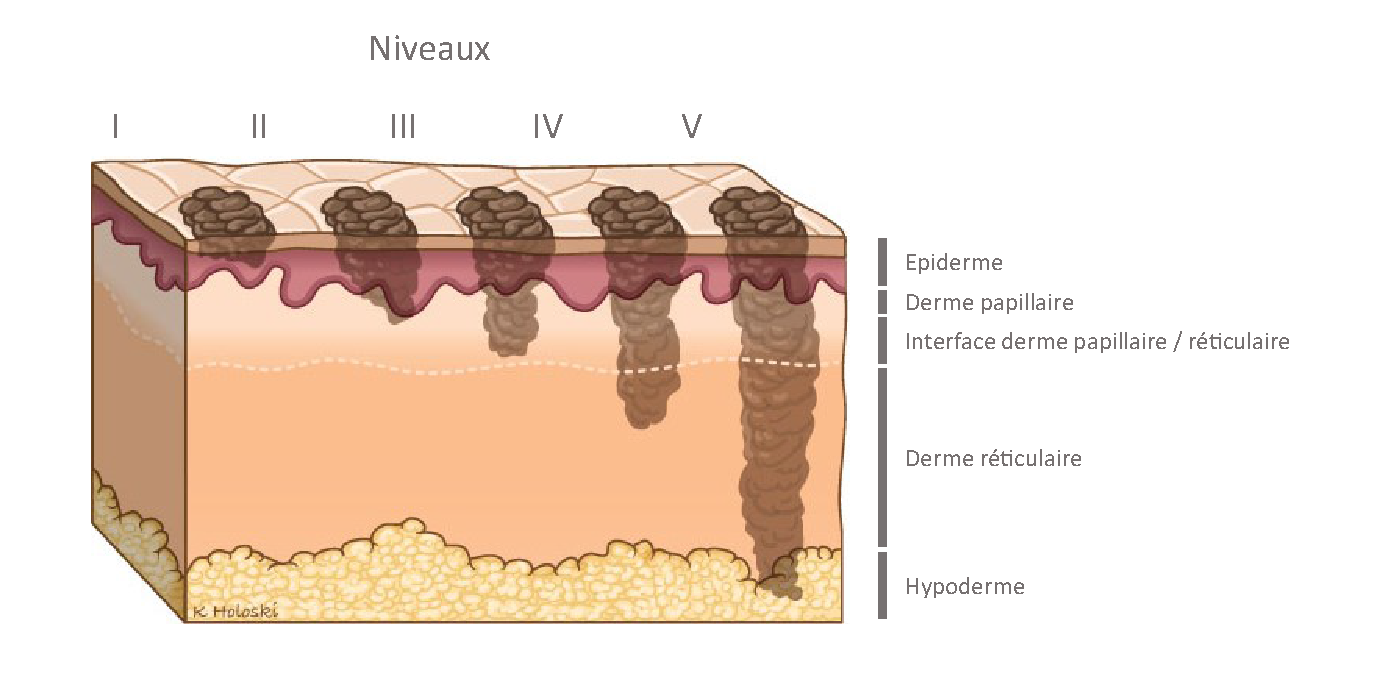
\includegraphics[width=0.9\linewidth]{contents/chapter_1/resources/illustration_clarklevels_kholoski.pdf}
    \caption{Illustration de l'indice de Clark~\cite{Clark1969}, défini par plusieurs niveaux de progression \textsuperscript{\ref{footnote:illustration_clarklevels_kholoski}}.}
    \label{fig:illustration_clarklevels_kholoski}
\end{figure}\par

\addtocounter{footnote}{1}
\footnotetext[\thefootnote]{Image source~: Dessin par \href{http://kholoski.com/}{Kellie Holoski} – Illustrateur médical. \label{footnote:illustration_clarklevels_kholoski}}

\subsubsection{Une pathologie particulière~: le Lentigo maligna}
\label{subsec:lentigo}
Les termes de \acrfull{lm} et de \acrfull{lmm} correspondent à des tumeurs qui touche les zones les plus exposées chez un individu tel que le visage chez les populations de plus de 60 ans. Comme précédemment énoncé, ils représentent environ 10\% des cas de mélanomes mais tendent à augmenter ces dernières années et vont désormais jusqu'à toucher les populations considérées comme jeunes. Le facteur explicatif le plus probable est l'exposition au soleil de plus en plus croissante chez ces différentes populations~\cite{Baccard2009, LeGal2011, LeDuff2014}.\par

Ainsi, le \textbf{\gls{lm}} résulte d'une prolifération de cellules malignes mélanocytaire au sein de la couche basale de l'épiderme, il s'agit d'un \textit{stade 0}, également considéré sous le terme de \textit{melanoma-in-situ}. Lorsque cette prolifération se propage aux cellules profondes de la peau au-delà de la \gls{dej} par le biais des follicules pileux, cette pathologie est alors qualifiée de \textbf{\gls{lmm}} et donne lieu à un risque important de métastases résultant de cette infiltration de cellules cancéreuses. Bien que la transition de \gls{lm} à \gls{lmm} soit souvent d'une dizaine d'années, il n'est pas isolé d'observer des cas dont l'évolution se fera entre deux examens bi-annuels~\cite{Mckenna2006, LeGal2011}. Les schémas propre au \gls{lm} et au \gls{lmm} sont observables sur la \Cref{fig:scheme_lm_stages}.\par

\begin{figure}[H]
    \centering
    \includegraphics[width=\linewidth]{example-image-a}
    \caption{}
    \label{fig:scheme_lm_stages}
\end{figure}\par

En termes de signes propre, le \gls{lm} se caractérise le plus souvent par une macules pigmentée, et par la présence de bordures et de pigmentations irrégulières et dont la taille atteint aisément une dizaine de centimètres. Le \gls{lmm} se présente sous la forme d'une lésion tumorale papuleuse ou nodulaire~\cite{Mckenna2006, LeGal2011}.\par

Les pathologies de \gls{lm} sont difficiles à diagnostiquer à l’œil nu et peuvent être confondues avec des pathologies bénignes telles qu'un \gls{sl}, une \gls{sk} ou une \gls{pak}~\cite{LeDuff2014}. Par ailleurs, les \gls{lm} sont très différents des autres types de mélanomes  et dont les limites peuvent être difficiles à définir. En effet, leur prolifération périphérique peut-être discrète voire non pigmentée~\cite{LeGal2011}.\par


Afin de lever cette ambiguïté, il est possible d'avoir recours à \textbf{l'histopathologie}. Le dermatologue procède à l'excision par biopsie d'un tissu intra-lésionnel considéré comme pathologique, puis ce même tissu est préparé afin d'être observé par microscope. D'une part, ce type de procédure est relativement long à réaliser et d'autre part représente une charge financière importante une fois rapporté au coût par examen. En addition, il s'agit d'une procédure incommodante pour le patient, pouvant échouer si le prélèvement est effectué en dehors d'un foyer mélanocytaire~\cite{LeGal2011}. Des exemples histologiques de pathologie de \gls{lm} peuvent être observés sur la \Cref{fig:example_lentigo_maligna} - en d) et e).\par

Cette difficulté à distinguer ces pathologies et les limitations induites par l'histopathologie conduisent à l'utilisation de dispositifs d'imagerie \textit{in-vivo} prévus pour ce domaine d'application. Ainsi, parmi les plus utilisés dans ce domaine peuvent être cités~:
\begin{inlinerate}
    \item la dermatoscopie,
    \item et la microscopie confocale par réflectance.
\end{inlinerate} Des exemples d'images de pathologies de \gls{lm} issues de ces dispositifs peuvent être observé sur la \Cref{fig:example_lentigo_maligna} - en a), b) et c). Le chapitre suivant s'oriente en ce sens en apportant des bases quant aux propriétés physiques de la peau et à la manière de l'observer.\par

% Des modèles de progression du stade ont été élaborés à partir d'observations par dermatoscopie comme présenté sur la \Cref{fig:illustration_surface_progression}.\par


% \begin{figure}[H]
%     \centering
%     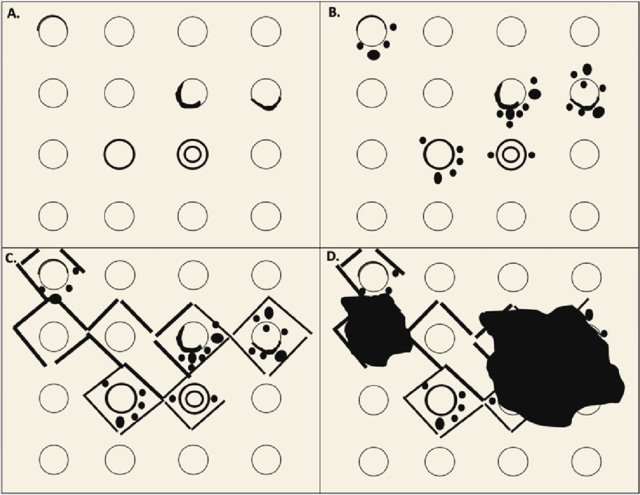
\includegraphics[width=0.7\linewidth]{contents/chapter_1/resources/illustration_surface_progression.jpg}
%     \caption{Modèle de progression horizontale observée par dermatoscopie~\cite{Navarrete-Dechent2020}. En a), ce stade est marqué par une agglomération et une ouverture asymétriques en périphérie des follicules pileux ; En b), ce stade est marqué par l'apparition de nervures et de schémas granuleux ; En c), ce stade est marqué par l'apparition de structures rhomboïdales ; En d) ce stade est marqué par des zones homogènes et une oblitération des ouvertures folliculaires.}
%     \label{fig:illustration_surface_progression}
% \end{figure}\par





\begin{figure}[H]
    \centering
    \includegraphics[width=\linewidth]{contents/chapter_1/resources/example_lentigo_maligna.pdf}
    \caption{Exemple d'une pathologie de \gls{lm} perçue à l'aide de différents dispositifs médicaux. En a), un aperçu par photographie clinique ; En b), un aperçu par dermatoscopie ; En c), un aperçu par Microscopie confocale par réflectance. En d) et e), les images fournissent un aperçu par histologie.}
    \label{fig:example_lentigo_maligna}
\end{figure}\par